\section{The Detection Service}
\label{sec:detection}

\subsection{Service Description}
\label{subsec:chdet_description}

This subsection describes the change detection service. Note that we have made several improvements compared to the specifications described in D3.1~\cite{d3.1}, which were dictated by interaction with the partners, efficiency reasons, or technical problems. The detailed description of these improvements are also included here. Familiarity with the contents of D3.1 is assumed.

\subsubsection{Change Types}

In Deliverable D3.1, we had defined four different levels of changes, namely low-level, basic, simple and complex.

Low-level changes represent changes at the triple level and constitute the basis upon which the detection process is based. As explained in D3.1, there are two low-level changes, namely \textit{add(t)} and \textit{delete(t)}, where \textit{t} is a triple. The detection of these changes uses the SPARQL queries described in Appendix~\ref{app:lowlevel} (cf. D3.1~\cite{d3.1}).

Basic changes were introduced as a layer to achieve completeness and unambiguity in the change detection process; in a nutshell, completeness guarantees that all changes that happen will be reported, whereas unambiguity guarantees that no change will be reported twice (see D3.1 for more details on these notions). 
Nevertheless, basic changes were subsequently dropped from our modelling , because the completeness and unambiguity could be easily guaranteed by the definition of simple changes. Therefore there was no longer need for basic changes. In addition, the removal of basic changes from our model made it simpler (three levels as opposed to four) and more efficient.

At the time of writing of Deliverable D3.1, simple changes were still vague; in the present deliverable, we provide the definitive listing of simple changes for the RDF and multidimensional models used by the pilots (see Appendix~\ref{app:simpleRDF} and~\ref{app:simpleMD}, respectively). The two listings are different, as different deployments (and data models) will use different simple changes. 
Both lists have been incorporated in the change detection service implementation.
These simple changes were defined in cooperation with the pilots, and are provably complete and unambiguous. Note that for each pilot, the corresponding set of simple changes should be predefined upon the deployment of the Change Detection module and it remains constant during the life-cycle of the module. Subsection~\ref{subsubsec:deploy} describes, among others, how the simple changes are predefined and ``passed" into the Change Detection module. 

Complex changes represent custom, user-defined changes, which are defined dynamically (at run-time) by the user. Complex changes are detected as described in D3.1. In this deliverable, we specify the information that the user should provide in order to define a complex change, and illustrate a mockup interface for this information to be submitted (see Subsection~\ref{subsec:chdet_tech} below). Even though this interface is not strictly under the hood of the change detection service (and WP3), we chose to describe it here for completeness.

\subsubsection{Assumptions}

The Change Detection module and its corresponding services were implemented under certain assumptions that are met by the DIACHRON model. These assumptions were agreed upon with the pilot partners and the partner ATHENA, who is responsible for the underlying storage model.

Firstly, the change detection module will consider datasets that were provided by the data pilots and have already been ingested and \emph{transformed} into the corresponding DIACHRON model in a complete and consistent way. For instance, the ontological data which are provided by EMBL were transformed, as dictated in Deliverable D4.1, into the corresponding DIACHRON model via Ontological-to-DIACHRON mappings. As a result, the Change Detection module is agnostic to the original pilot's data and their internal representation. 

One more assumption we considered during the implementation phase is the form that the object URIs should have within DIACHRON platform. More specifically, we assumed that URIs are constructed in such way that when we refer on the ``same" objects (i.e., classes, properties) across different versions, their URIs will remain persistent as well. 
Thus, an entity retains the same URI across different versions, thereby being dereferenceable across all versions. Note that this is required for all pilots.
This feature is achieved via the transformation mechanism from the original pilots' datasets to DIACHRON data by ignoring the datasets' version numbers during the transformation process.

\subsubsection{Complex Changes Definition Interface}
\label{subsubsec:complex}

In this subsection, we describe the required input for managing complex changes.
We first focus on the most important operation of creating (i.e., defining) a complex change, and then discuss other operations (namely, deleting and editing complex changes). In all cases, we explain what is the required input that the user interface should provide in order to allow the change detection service to manipulate the corresponding change. The mockup for providing this information appears in~\ref{subsec:chdet_tech}.

\paragraph{Creating Complex Changes}

When creating a new complex change, the following information should be requested via the user interface and provided to the internal function that creates the complex change:

\begin{description}

\item[Name:] A descriptive name for the complex change (mandatory). Names of changes should be unique, i.e., a new complex change could not have the same name as a previously defined simple or complex change.

\item[Priority:] A float number denoting the priority of the change (to help solve ambiguities during the change detection phase -- cf. D3.1~\cite{d3.1}); this is also mandatory.

\item[Parameter Names:] An ordered set of parameters, defined through their descriptive names (and denoted by $P^*_1, \dots,$ $P^*_n$).
Parameter names should be unique within each change, but it is possible for different (simple or complex) changes to share the same parameter name.
It is allowed, though not recommended, for this set to be empty, i.e., for a change to have no parameters.

\item[Mandatory Simple Changes:] A set of selected simple change(s) over the total set of simple changes per pilot deployment, that comprise the specified complex change. Note that each simple change has a name ($S_1,\dots,S_m$), as well as its own parameters ($P_{ij}$, denoting the $j^{th}$ parameter of $S_i$). There must be at least one mandatory simple change.

\item[Optional Simple Changes:] A set of selected simple change(s) over the total set of simple changes per pilot deployment that could be optionally ``consumed'' during the detection of the specified complex change. It is possible that there are no optional simple changes.

\item[Parameter Filters:] For each parameter $P^*_k$ of the complex change, we should apply a selection filter (equality operator) over a simple change parameter $P_{ij}$. 
Thus, a parameter filter is of the form: $P^*_k = P_{ij}$, where $P^*_k$, $P_{ij}$ are the names for the complex change parameter and simple change parameter, respectively; note that the simple change could be mandatory or optional. 
This filter associates a complex change parameter with a simple change parameter. 
%This filter indicates where each parameter of the complex change takes its value from. 
Parameter filters are mandatory, i.e., there should be exactly one parameter filter per complex change parameter.

\item[Selection Filters:] Different types of selection filters on specified parameters could be optionally added by the user. 
These should have the form $P_{ij}$ $\ast$ $X$ where $\ast$ can be any SPARQL comparison operator (e.g., $=$, $>$ etc.) and $X$ can be any URI or literal supported by SPARQL.

\item[Join Filters:] Additionally, join filters across different parameters of simple changes can be optionally added. 
These should be of the form $P_{ij} = P_{i'j'}$, where $P_{ij}, P_{i'j'}$ are different parameter names of the mandatory or optional simple changes comprising the complex one.

\item[Mapping Filters:] Some complex changes are based on \textit{mappings} that express that two different URIs (in different versions) represent the same real-world concept; this is necessary to encode certain types of changes, such as those that represent rename, merge or split operations. 
To express the fact that such a mapping should exist for a complex change to be detectable, mapping filters are introduced. Such filters may have one of the following forms: 
$P_{ij} \rightarrow P_{i'j'}$ or
$P_{ij} \rightarrow \{P_{i'_1 j'_1}, \dots, P_{i'_n j'_n}\}$ or
$\{P_{i_1 j_1}, \dots, P_{i_n j_n}\} \rightarrow P_{i'j'}$.
Note that not all complex changes have mapping filters, i.e., this field is optional.

\item[Version Filters:] These filters are used to (optionally) express conditions over triples or URIs that should (or should not) exist in the old and/or the new version. Such filter(s) can be of one of the following forms: 
``$x$ IN $V$'' or ``$x$ NOT IN $V$'' where $x$ can be either a URI or a triple, and $V$ can be either the old or the new version (denoted by $V_{old}, V_{new}$ respectively).

\end{description}

All the above filters are understood conjunctively, but filters combined via disjunction (or a combination of disjunction and conjunction) are also technically possible.
However, it is an open issue whether this functionality could be useful for the user, as we believe that this sophisticated version could overwhelm the user with many options. 
For this reason, disjunctive filters are not supported in this version of the implementation, but their usability will be evaluated in the near future in order to determine whether to include this functionality in the next version of the implementation.



\begin{example}
The following is an intuitive example which will help to visualize and better understand the process, via clarifying how the above input requirements can be materialized to define a complex change.
In particular, we will define the change ``Mark as Obsolete'', which is used to encode/capture a standard pattern of changes that the EBI pilot uses when they want to delete a class; in this case, the class is not physically deleted, but marked as ``obsolete'', via a label. Formally, the change can be defined as follows:
\begin{description}
%\item [Complex Change Example:] Mark as obsolete
\item [Name:] Mark as Obsolete
\item [Priority:] 2
\item [Parameter Names:] obs\_class, obs\_reason
\item [Mandatory Simple Changes:] Add\_Superclass(subclass, superclass)
\item [Optional Simple Changes:] Add\_Label(class, label), Add\_Property\_Instance(subj, prop, obj)
\item [Parameter Filters:] obs\_class = subclass, obs\_reason = obj
\item [Selection Filters:] superclass = ``ObsoleteClass", prop = ``reason\_for\_obsolescence"
\item [Join Filters:] class = subclass, subj = subclass 
\item [Mapping Filters:] -
\item [Version Filters:] -
\end{description}
\end{example} 

\paragraph{Deleting Complex Changes}
When deleting a complex change, all we need is the name of the deleted complex change. The deletion of a complex change eliminates all references of said change from the ontology of changes, including previous detections.

\paragraph{Editing Complex Changes}
In this version, editing a complex change is implemented as a deletion followed by a creation of a change. In the second version of the DIACHRON platform (due on M28), we will consider a more efficient implementation.

\subsubsection{Ontology of Changes}

Ontologies provide the functionality of maintaining (sharing and reuse) linked datasets and allow the flexible tracking of changes with support of query capabilities in a uniform manner. In addition, the ontological representation provides a supervisory look of the detected changes (either simple or complex) and their association with the entities they refer to in the actual datasets. Moreover, this representation provides useful information about the definition of changes. 

Based on this motivation, in Deliverable D3.1~\cite{d3.1}, we described an \textit{ontology of changes} for storing the detected changes in a convenient format, which allows the 
association of information on the changes with the actual data; this ability is the cornerstone for supporting cross-snapshot queries, for supporting queries that deal with both the data and the changes, and for treating changes as first-class citizens. 
An additional role for the ontology of changes is to provide a storage mechanism for the definitions (i.e., specifications) of the user-defined complex changes.

Since the delivery of D3.1 in M12 of the project, the ontology of changes underwent certain revisions, dictated by technical problems identified, feedback from pilots and other partners, as well as by the revisions performed in the structure of changes that were described above. 
Below, we list the revisions made on the ontology of changes as compared to 
what was reported in D3.1; the new version of the ontology is visualized in Figures~\ref{fig:mappings}-~\ref{fig:cc detection}:

\begin{figure}[t]
\centering
\includegraphics[width=100mm]{figures/mappings.png}
\caption{Mappings Representation}
\label{fig:mappings}
\end{figure}

\begin{figure}[t]
\centering
\includegraphics[width=100mm]{figures/mappings_instances.png}
\caption{Example of a Mapping Representation}
\label{fig:mappings_inst}
\end{figure}

\begin{figure}[H]
\centering
\includegraphics[width=120mm]{figures/Slide1.PNG}
\caption{Top-level Concepts}
\label{fig:ontology of changes overview}
\end{figure}

\begin{figure} [h]
	\centering
    \begin{subfigure}[b]{0.7\textwidth}
		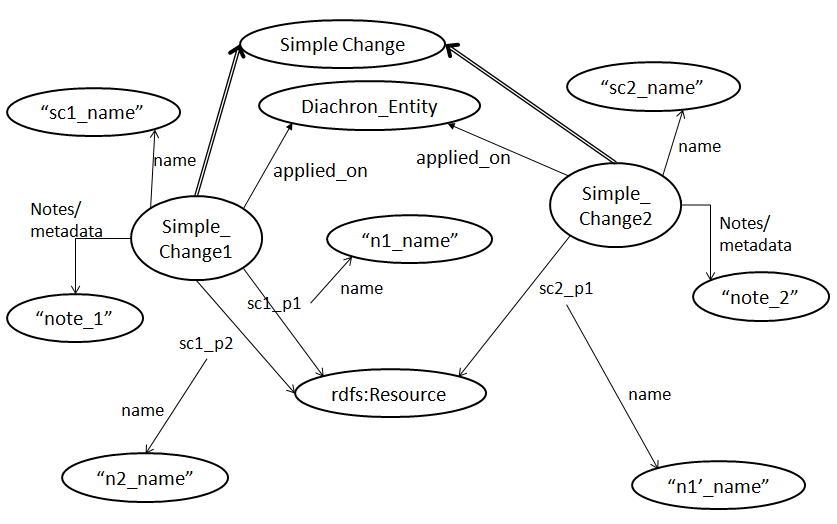
\includegraphics[width=\textwidth]{figures/Slide4.PNG}
	    \caption{General Case}
        \label{fig:simple changes}
    \end{subfigure}
        \begin{subfigure}[b]{0.7\textwidth}
        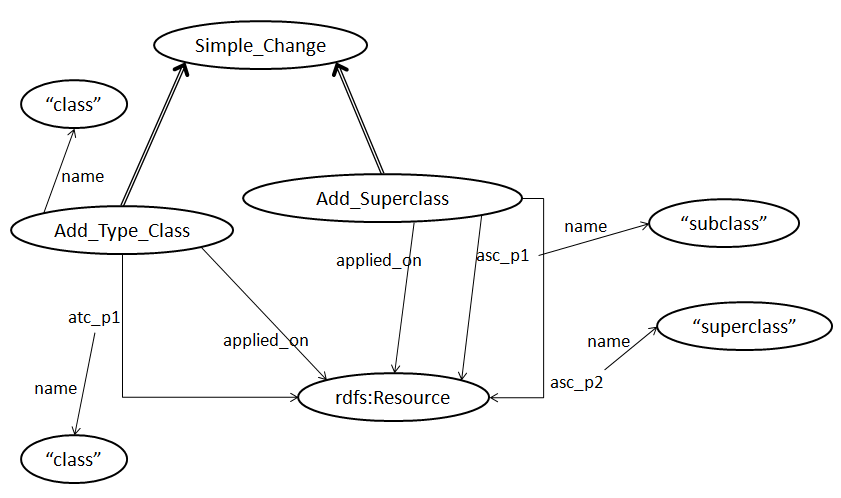
\includegraphics[width=\textwidth]{figures/Slide5.PNG}
        \caption{Example of the Definition of Two Sample Simple Changes}
        \label{fig:ebi simple changes}
	\end{subfigure}
    \caption{Ontological Structures for Representing the Definition of Simple Changes}
    \label{fig:simplchan}
\end{figure}

\begin{figure}[t]
\centering
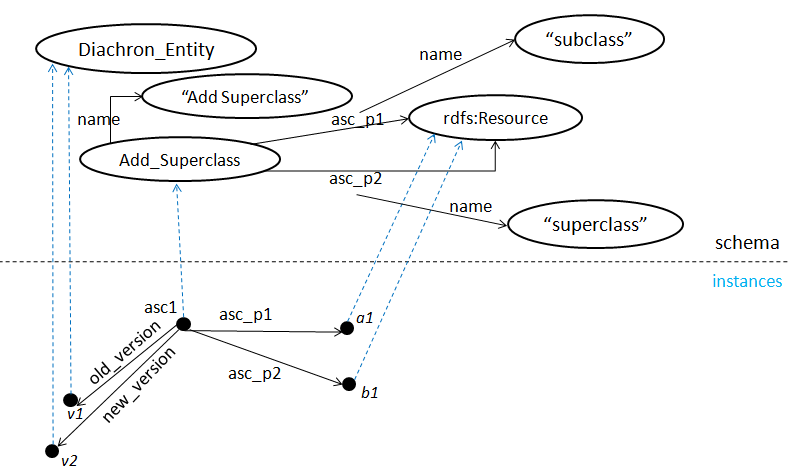
\includegraphics[width=120mm]{figures/Slide6.PNG}
\caption{Simple Changes Detection}
\label{fig:sc detection}
\end{figure}

\begin{figure} [t]
	\centering
    \begin{subfigure}[b]{0.7\textwidth}
		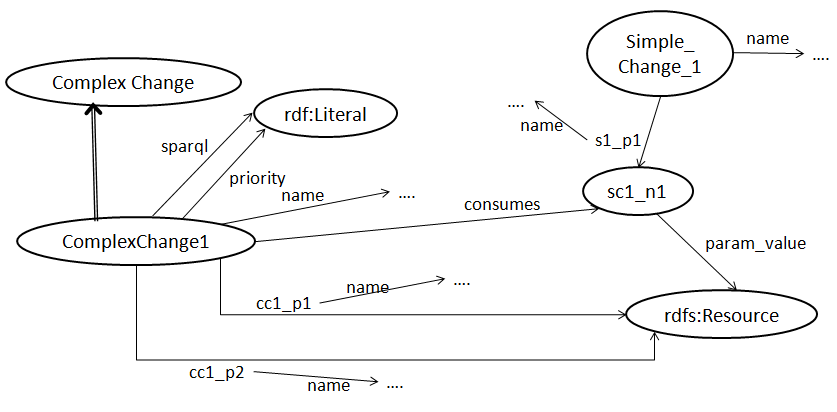
\includegraphics[width=\textwidth]{figures/Slide7.PNG}
	    \caption{General Case}
        \label{fig:cc example}
    \end{subfigure}
        \begin{subfigure}[b]{0.7\textwidth}
        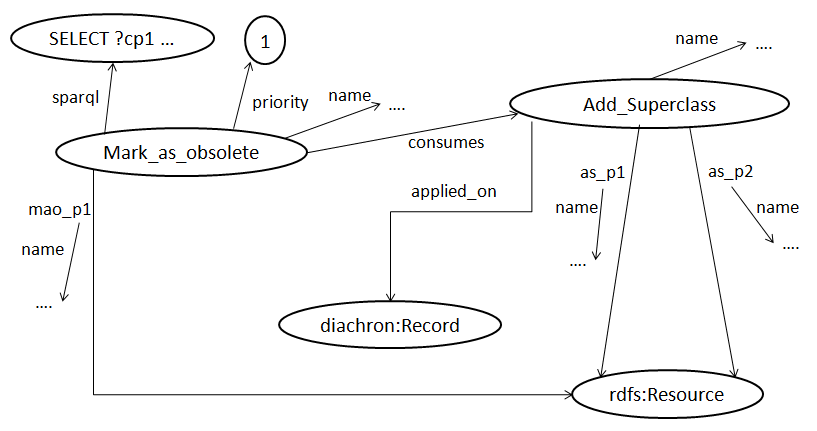
\includegraphics[width=\textwidth]{figures/Slide8.PNG}
        \caption{Example of the Definition of a Complex Change}
        \label{fig:cc_definition}
	\end{subfigure}
    \caption{Ontological Structures for Representing the Definition of Complex Changes}
    \label{fig:comchan}
\end{figure}

\begin{figure}[t]
\centering
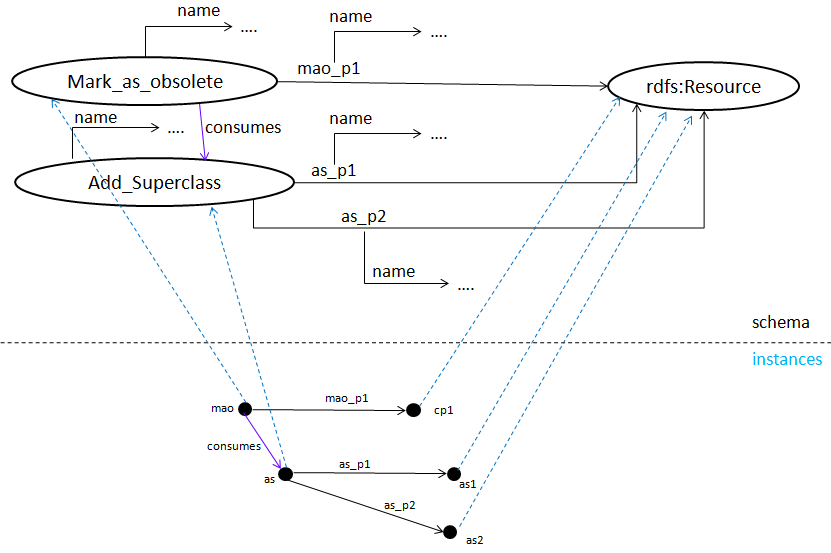
\includegraphics[width=120mm]{figures/Slide9.PNG}
\caption{Complex Change Detection}
\label{fig:cc detection}
\end{figure}

\begin{enumerate}

\item As basic changes were dropped from our modelling, they were also dropped from the ontology (see Figure~\ref{fig:ontology of changes overview}).

\item For each simple and complex change, as well as for each simple and complex change parameter, we added a property named \textit{"name"} to hold a user defined descriptive name 
(see Figures~\ref{fig:simplchan}-\ref{fig:cc detection}); 
this was necessary to allow a more intuitive interaction with the user during the construction of a complex change.
For the parameter names in particular, the \textit{"name"} property has as domain the property that connects the parameter with its value (see Figures~\ref{fig:simplchan}-\ref{fig:cc detection}); this was done for efficiency purposes.

\item The \textit{``consumes"} property was added to denote the fact that certain simple changes are subsumed by complex ones (in technical terms, the detection of a complex change consumes said simple changes -- cf.~\cite{d3.1} and 
Figures~\ref{fig:comchan},~\ref{fig:cc detection}).

\item We simplified the representation of the definition of complex changes, keeping only the information that is absolutely relevant and critical for the system. In particular, the properties 
\textit{"refers\_to"}, \textit{"visible"}, \textit{"filter"}, \textit{"comprise\_of\_mand"} and \textit{"comprise\_of\_opt"} were dropped, because the information they represent was embedded in the SPARQL query which is used for the detection of said complex change (see Figures~\ref{fig:comchan},~\ref{fig:cc detection}).

\item A generic \textit{"notes/metadata"} property was added to changes. This property is not used at this stage, but is reserved for future use in order to store notes related to the change such as an intuitive description, or provenance information.

\item We enhanced the ontology, so as to be able to store mappings between URIs residing in different versions of datasets; these are necessary for the definition of some complex changes that
represent rename, merge or split operations (cf. Subsection~\ref{subsubsec:complex}). 
Mappings are stored as instances of a new class called \textit{"Map"}, as shown in Figure~\ref{fig:mappings}. 
We use the properties \textit{"old\_version"}, \textit{"new\_version"} to denote in which dataset versions a mapping refers to, and the properties \textit{"old\_value"}, \textit{"new\_value"} to link the URI(s) in the old and new version. 
Moreover, we provide the property \textit{"notes/metadata"} (as with changes) to store any high level information related to the mappings (e.g., notes, provenance etc).
An example of storing mappings is illustrated in Figure~\ref{fig:mappings_inst}, the left part of which shows a one-to-one mapping ($x1 \rightarrow x2$) from $v1$ to $v2$ (useful for renames), 
whereas the right part shows a one-to-many mapping ($y1 \rightarrow \{y2,y3\}$) from $v1$ to $v2$ (useful for splits).

\item We replaced some classes that functioned as ranges for certain properties with more generic ones; in particular, for generic RDF resources, related to data, the classes \textit{"rdfs:Class"}, \textit{"rdf:Property"} etc were replaced by the more general \textit{"rdfs:Resource"}, and the new class \textit{"diachron:Entity"} was used as a generic container for DIACHRON entities (see Figures~\ref{fig:simplchan}-~\ref{fig:cc detection}).

\item The central class \textit{Change} of the ontology was defined to be a subclass of \textit{prov:activity} (see the upcoming Deliverable D2.2, due on M16).

\end{enumerate}

\subsubsection{Querying Changes}

As mentioned above, the ontology of changes was introduced in order to allow the user to perform queries on both the data and the changes, thereby treating changes as first-class citizens, which is one of the main objectives of DIACHRON.
To support the user in this task, we created a method allowing query access to the ontology of changes. 
This $GET$ method is implemented within service \emph{\//diachron\//change\_detection} and requires the following parameters:
\begin{enumerate}
	\item the SPARQL query which will be applied upon the ontology of changes
	\item the format of the query results i.e., xml, csv, tsv, json
\end{enumerate}
More details on this method can be found in Subsection~\ref{subsec:chdet_tech}.
